\section*{Exercice 189 -- Modélisation}
\setcounter{exo}{0}
%E3A MP 2009

Le vérin du système presseur est implanté entre le bâti fixe de la machine et le
support du rouleau presseur.

\begin{center}
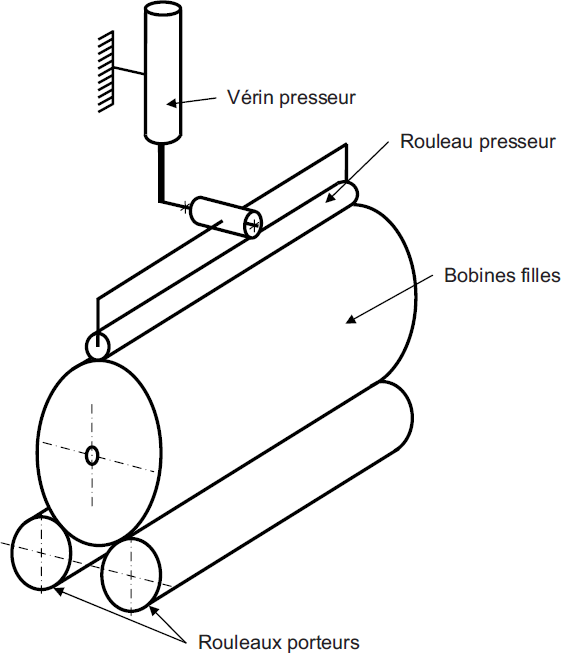
\includegraphics[width=.5\linewidth]{987_01}%
\end{center}

L’asservissement en effort de ce système est réalisé par une servovalve qui permet de
réguler la pression et le débit du fluide d’alimentation des vérins.
Un système de capteurs de pression permet d’assurer la mesure pour cet asservissement.
La figure suivante donne la chaîne fonctionnelle de cet asservissement en effort.

\begin{center}
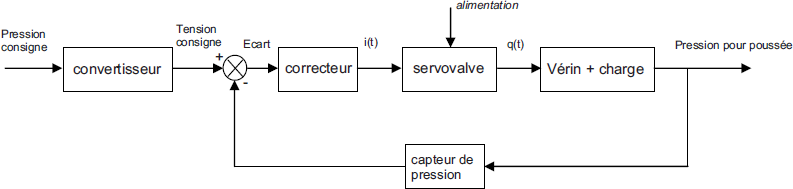
\includegraphics[width=\linewidth]{987_02}%
\end{center}

La figure suivante présente un schéma simplifié du système hydraulique au niveau de la
servovalve.

\begin{center}
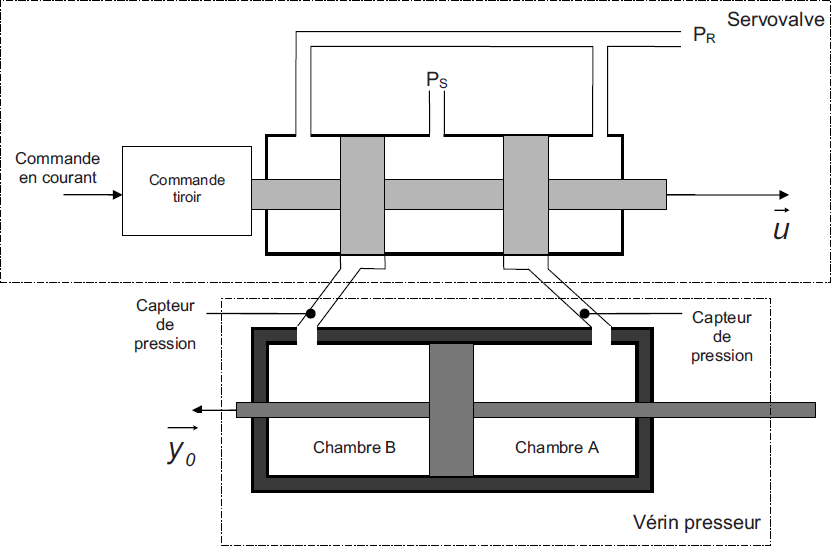
\includegraphics[width=\linewidth]{987_03}%
\end{center}


\subsubsection*{Notation}
\begin{itemize}
\item $P_S$ : pression de service ;
\item $P_R$ : pression de refoulement ;
\item $p_A(t)$ et $p_B(t)$ : pression dans les chambres $A$ et $B$ du vérin ;
\item $V_A$ et $V_B$ : volume des chambres $A$ et $B$ du vérin ;
\item $q_A(t)$ et $q_B(t)$ : débit d’alimentation des chambres $A$ et $B$ du vérin ;
\item $ \nu$  : coefficient de frottement visqueux de l’huile ;
\item $S$ : section utile du piston du vérin ;
\item $f(t)$ : effort développé par le vérin ;
\item $i(t)$ : commande de courant de la servovalve;
\item $y(t)$ : position du piston de la tige du vérin selon l’axe $\vect{y_0}$.
\end{itemize}

Pour l’ensemble du sujet, les variables de Laplace seront notées en majuscule, et les
variables temporelles seront en minuscule. Exemple $L[f(t)] = F(p)$.


\subsubsection*{Fonctionnement}
Par une commande en courant $i(t)$ positive, on déplace le tiroir dans le sens de $\vect{u}$ positif. La
pression dans la chambre $A$ va alors augmenter et celle dans la chambre $B$ va diminuer.
La différence de pression $(p_A(t)– p_B(t))$ génère alors un déplacement de la tige du vérin dans
le sens de $\vect{y_0}$ positif.

\subsubsection*{Hypothèses de travail}
\begin{itemize}
\item L’huile est supposée compressible, cela se traduit par la relation suivante : $\dfrac{\Delta v}{v} = -\dfrac{\Delta p}{B}$ avec $v$ volume du fluide, $p$ pression du fluide, $B$ module de compressibilité; 
\item Le distributeur a un comportement symétrique ce qui implique qu’au repos, en
l’absence de charge, la pression dans chaque chambre est supposée égale à $P_S/2$.
\end{itemize}

\subsubsection*{Modélisation de la servovalve}
\begin{center}
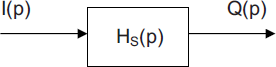
\includegraphics[width=.5\linewidth]{987_04}%
\end{center}

Un essai constructeur en réponse indicielle unitaire sur la servovalve donne la
caractéristique suivante.

\begin{center}
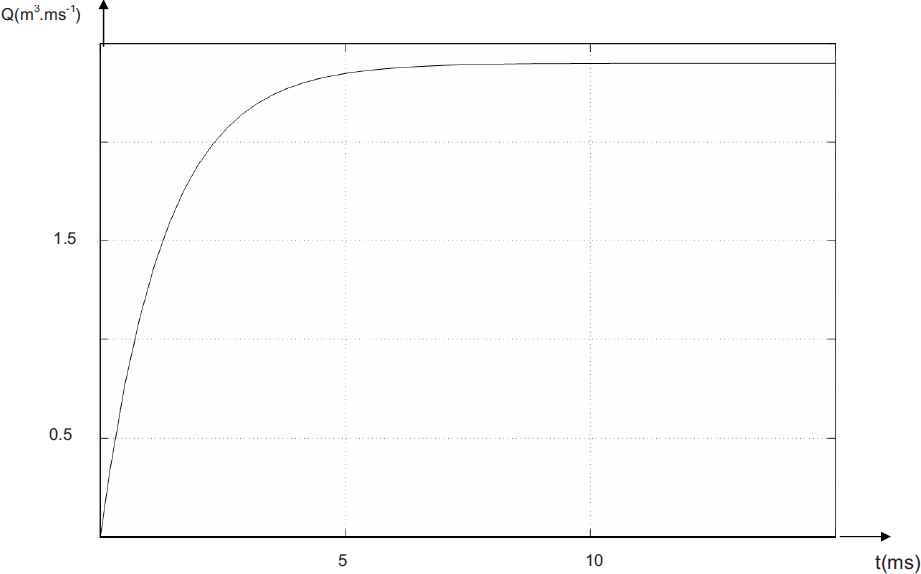
\includegraphics[width=\linewidth]{987_05}%
\end{center}


\subparagraph{}
\textit{Donner les valeurs caractéristiques $K_S$ et $T_S$ de la
servovalve. Vous préciserez les valeurs numériques ainsi que les unités.
Compléter le bloc correspondant sur le schéma-blocs.}
\ifprof
\begin{corrige}
\end{corrige}
\else
\fi


\begin{center}
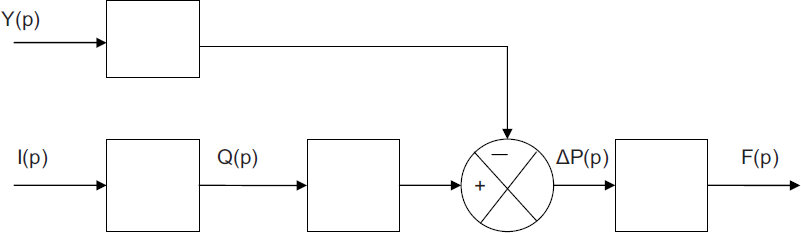
\includegraphics[width=\linewidth]{987_06}%
\end{center}

\subsubsection*{Approche simplifiée : modélisation du vérin seul}
Le débit étant faible, on négligera la viscosité de l’huile dans cette partie.

\subparagraph{}
\textit{Donner, dans le domaine temporel, l’expression littérale de l’effort développé par le vérin.}
\ifprof
\begin{corrige}
\end{corrige}
\else
\fi

\subparagraph{}
\textit{En supposant les conditions initiales nulles, exprimer dans le domaine de Laplace
l’équation établie à la question précédente. Compléter alors le schéma-blocs.}
\ifprof
\begin{corrige}
\end{corrige}
\else
\fi

On donne l’expression littérale du débit $q_A(t)$ dans la chambre $A$ du vérin :
$q_A(t)=S\dfrac{\dd y(t)}{\dd t}+\dfrac{V_A}{B}\dfrac{\dd p_A(t)}{\dd t}$.

Le premier terme de cette expression $S\dfrac{\dd y(t)}{\dd t}$ correspond au débit engendré par le
déplacement du piston du vérin. Le deuxième terme $\dfrac{V_A}{B}\dfrac{\dd p_A(t)}{\dd t}$ est dû à la compressibilité
du fluide.

\subparagraph{}
\textit{Déterminer l’expression littérale reliant le débit $q_B(t)$, la pression $p_B(t)$ dans la
chambre $B$, le déplacement de la tige $y(t)$, et les paramètres du système.}
\ifprof
\begin{corrige}
\end{corrige}
\else
\fi


On suppose pour la suite de l’étude que le vérin se trouve au voisinage de sa position
médiane, ce qui permet de supposer que $V_A = V_B = V$.
De plus, on pose $p_A(t) – p_B(t)= \Delta p(t)$ et $q_A(t) = -q_B(t) = q(t)$.


\subparagraph{}
\textit{À partir des nouvelles données et des expressions précédentes, déterminer la
relation littérale liant  $p(t)$, $y(t)$, $q(t)$, et les paramètres du système.}
\ifprof
\begin{corrige}
\end{corrige}
\else
\fi

\subparagraph{}
\textit{En supposant les conditions initiales nulles, exprimer dans le domaine de Laplace
l’équation précédente.
Compléter alors le schéma bloc du document réponse DR4.}
\ifprof
\begin{corrige}
\end{corrige}
\else
\fi

\begin{enumerate}
\item $K_S = \SI{2,4}{m^3.ms^{-1}.A^{-1}}$ et $T_S = \SI{1,5}{ms}$.
\item $f(t)=\left(p_A(t)-p_B(t)\right)S$.
\item $F(p)=\left(P_A(p)-P_B(p)\right)S=\Delta (p)S$.
\item $q_B(t)=-S\dfrac{\dd y(t)}{\dd t}+\dfrac{V_B}{B}\dfrac{\dd p_B(t)}{\dd t}$
\item $q(t)=S\dfrac{\dd y(t)}{\dd t}+\dfrac{V}{2B}\dfrac{\dd \Delta p(t)}{\dd t}$
\item $Q(p)=SpY(p)+\dfrac{V}{2B}\Delta P (p)$
\end{enumerate}
